\documentclass[../master/master.tex]{subfiles}

\begin{document}

%----------------------------------------------------------------------
% LECTURE 4: Topic
% Date: January 29, 2026
%----------------------------------------------------------------------
\renewcommand{\lecturenum}{4}
\renewcommand{\lecturedate}{January 29, 2026}
\renewcommand{\lecturetopic}{Topological Spaces, Metric Topology}

\section{Lecture \lecturenum : \lecturedate}

\begin{lecturesummary}
\textbf{Lecture Overview:} We introduce the abstract notion of a topological space and its key building blocks: open sets, bases, and the topology they generate. We then specialize to metric spaces, where open balls form a natural basis, and develop the metric topology with epsilon-delta techniques. Finally, we study closed sets, closures, and limit points --- the dual perspective to open sets --- along with boundedness, convexity, convergence, and the equivalence of the product and metric topologies on $\R^n$.
\medskip
\begin{center}
\begin{tabular}{c l}
\hline
\textbf{Symbol} & \textbf{Meaning} \\
\hline
$\mathcal{T}$ & A topology (collection of open sets) on $X$ \\
$\mathcal{B}$ & A basis for a topology \\
$(X, d)$ & A metric space (set $X$ with metric $d$) \\
$B(x, \eps)$ & Open ball of radius $\eps$ centered at $x$ \\
$E$ & A subset of $X$ \\
$\overline{E}$ & Closure of $E$ (smallest closed set containing $E$) \\
$E'$ & Derived set (set of all limit points of $E$) \\
$E \setminus E'$ & Isolated points of $E$ \\
Open set & A set $U \in \mathcal{T}$; every point has a neighborhood inside $U$ \\
Closed set & Complement of an open set; contains all its limit points ($E' \subseteq E$) \\
\hline
\end{tabular}
\end{center}
\end{lecturesummary}

\subsection{Topological Spaces}

\begin{summarybox}
\textbf{Section Overview:} We define a topology on a set $X$ via three axioms governing open sets, then explore examples (discrete and cofinite topologies). We introduce the notion of a basis for a topology and show that every open set is a union of basis elements.
\end{summarybox}

\begin{definition}
A \defn{topology} on a set $X$ is a collection $\mathcal{T}$ of subsets of $X$ such that:
\begin{enumerate}
    \item $\emptyset \in \mathcal{T}$ and $X \in \mathcal{T}$.
    \item For all $\mathcal{S} \subseteq \mathcal{T}$, $\displaystyle\bigcup_{S \in \mathcal{S}} S \in \mathcal{T}$ (arbitrary unions).
    \item If $\mathcal{S} \subseteq \mathcal{T}$ is finite, then $\displaystyle\bigcap_{S \in \mathcal{S}} S \in \mathcal{T}$ (finite intersections).
\end{enumerate}
\end{definition}

\begin{remark}
The elements of $\mathcal{T}$ are called \defn{open sets}.
\end{remark}

\begin{example}
The \defn{discrete topology} on a set $X$ is $\mathcal{T} = \mathcal{P}(X)$, the power set of $X$. In this topology, every subset of $X$ is open. For instance, $\Z \subseteq \R$ inherits the discrete topology from the standard topology on $\R$: every subset of $\Z$ is open.
\end{example}

\begin{notebox}
\textbf{Why is $\Z$ discrete in $\R$?} For any $n \in \Z$, the interval $(n - \frac{1}{2}, n + \frac{1}{2}) \cap \Z = \{n\}$, so every singleton $\{n\}$ is open in the subspace topology on $\Z$. Since arbitrary unions of open sets are open, every subset of $\Z$ is open. Intuitively, the integers are ``isolated'' --- there is space around each one with no other integers nearby. The discrete topology is the topology where every set is open, which is the finest (most open sets) possible topology on a set.
\end{notebox}

\begin{example}
The \defn{finite-complement topology} (or cofinite topology) on a set $X$: a subset $U \subseteq X$ is open if and only if $X \setminus U$ is finite (or $U = \emptyset$).

We verify the three topology axioms:
\begin{enumerate}
    \item $\emptyset$ is open by convention. $X$ is open since $X \setminus X = \emptyset$ is finite.
    \item Let $\{U_\alpha\}_{\alpha \in A}$ be a collection of open sets. Then
    \[
        X \setminus \bigcup_{\alpha \in A} U_\alpha = \bigcap_{\alpha \in A} (X \setminus U_\alpha).
    \]
    Each $X \setminus U_\alpha$ is finite, so the intersection is a subset of any one of them, hence finite. Thus $\bigcup U_\alpha$ is open.
    \item Let $U_1, \dots, U_n$ be finitely many open sets. Then
    \[
        X \setminus \bigcap_{i=1}^{n} U_i = \bigcup_{i=1}^{n} (X \setminus U_i).
    \]
    Each $X \setminus U_i$ is finite, and a finite union of finite sets is finite. Thus $\bigcap_{i=1}^n U_i$ is open.
\end{enumerate}
\end{example}

\begin{notebox}
\textbf{How does this relate to shapes like a torus?} The axioms above define topology in full generality --- they tell us what it means for sets to be ``open'' without any reference to distance or geometry. A shape like a torus is a \emph{topological space}: a set of points (the surface) equipped with a topology (which subsets count as open). Two shapes are ``the same'' topologically if there is a continuous bijection with a continuous inverse (a homeomorphism) between them. The famous ``coffee mug = donut'' equivalence means there is such a map between them. The abstract axioms here are the foundation: they capture exactly the structure needed to define continuity, connectedness, and compactness, which are the properties that let us distinguish a torus from a sphere without ever measuring distances or angles.

\begin{center}
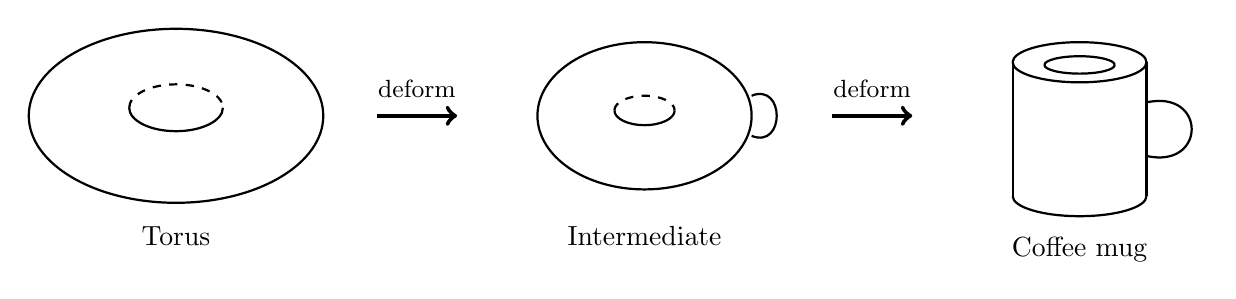
\begin{tikzpicture}[scale=0.85]
    % Torus
    \draw[thick] (0,0) ellipse (2.2 and 1.3);
    \draw[thick] (-0.7,0.12) arc (180:360:0.7 and 0.35);
    \draw[thick, dashed] (-0.7,0.12) arc (180:0:0.7 and 0.35);
    \node at (0,-1.8) {Torus};

    % Arrow 1
    \draw[->, ultra thick] (3,0) -- (4.2,0);
    \node at (3.6,0.4) {\small deform};

    % Intermediate
    \begin{scope}[xshift=7cm]
        \draw[thick] (0,0) ellipse (1.6 and 1.1);
        \draw[thick] (-0.45,0.08) arc (180:360:0.45 and 0.22);
        \draw[thick, dashed] (-0.45,0.08) arc (180:0:0.45 and 0.22);
        \draw[thick] (1.6,0.3) .. controls (2.1,0.5) and (2.1,-0.5) .. (1.6,-0.3);
        \node at (0,-1.8) {Intermediate};
    \end{scope}

    % Arrow 2
    \draw[->, ultra thick] (9.8,0) -- (11,0);
    \node at (10.4,0.4) {\small deform};

    % Coffee mug
    \begin{scope}[xshift=13.5cm]
        \draw[thick] (-1,-1.2) -- (-1,0.8);
        \draw[thick] (1,-1.2) -- (1,0.8);
        \draw[thick] (-1,0.8) arc (180:360:1 and 0.3);
        \draw[thick] (-1,0.8) arc (180:0:1 and 0.3);
        \draw[thick] (-1,-1.2) arc (180:360:1 and 0.3);
        \draw[thick] (1,0.2) .. controls (1.9,0.4) and (1.9,-0.8) .. (1,-0.6);
        \draw[thick] (-0.525,0.76) arc (180:360:0.525 and 0.13);
        \draw[thick] (-0.525,0.76) arc (180:0:0.525 and 0.13);
        \node at (0,-2.0) {Coffee mug};
    \end{scope}
\end{tikzpicture}

\smallskip
\small Both have exactly one hole --- they are homeomorphic (genus 1 surfaces).
\end{center}
\end{notebox}

\begin{definition}
A \defn{basis} for a topology on $X$ is a collection $\mathcal{B}$ of subsets of $X$ such that:
\begin{enumerate}
    \item For all $x \in X$, there exists $B \in \mathcal{B}$ such that $x \in B$.
    \item For all $B_1, B_2 \in \mathcal{B}$ and for all $x \in B_1 \cap B_2$, there exists $B_3 \in \mathcal{B}$ with $B_3 \subseteq B_1 \cap B_2$ and $x \in B_3$.
\end{enumerate}
\end{definition}

The \defn{topology generated by $\mathcal{B}$} is defined as follows: $U \in \mathcal{T}$ if and only if for all $x \in U$, there exists $B \in \mathcal{B}$ such that $x \in B$ and $B \subseteq U$.

\begin{example}
The \defn{order topology} on $\R$ is generated by the basis of open intervals $(a, b)$ for $a < b$.
\end{example}

\begin{lemma}
Let $\mathcal{B}$ be a basis for the topology $\mathcal{T}$ on $X$. Then $\mathcal{T}$ equals the collection of all unions of elements of $\mathcal{B}$.
\end{lemma}

\begin{proof}
Let $\mathcal{U}$ denote the collection of all unions of elements of $\mathcal{B}$. We show $\mathcal{T} = \mathcal{U}$.

$(\supseteq)$ Each $B \in \mathcal{B}$ is open (since for any $x \in B$, the element $B$ itself witnesses $x \in B \subseteq B$). Since $\mathcal{T}$ is closed under arbitrary unions, every union of elements of $\mathcal{B}$ is in $\mathcal{T}$. Thus $\mathcal{U} \subseteq \mathcal{T}$.

$(\subseteq)$ Let $U \in \mathcal{T}$. For each $x \in U$, by definition of the topology generated by $\mathcal{B}$, there exists $B_x \in \mathcal{B}$ with $x \in B_x \subseteq U$. Then
\[
    U = \bigcup_{x \in U} B_x,
\]
which is a union of elements of $\mathcal{B}$. Thus $U \in \mathcal{U}$, so $\mathcal{T} \subseteq \mathcal{U}$.
\end{proof}

\subsection{Metric Topology}

\begin{summarybox}
\textbf{Section Overview:} We define metrics, open balls, and the metric topology they generate. Key results include the characterization of open sets via epsilon-balls, the product topology equaling the metric topology on $\R^n$, and the epsilon-delta proof technique that recurs throughout analysis.
\end{summarybox}

\begin{definition}
Let $X$ and $Y$ be topological spaces. The \defn{product topology} on $X \times Y$ is the topology generated by the basis
\[
    \mathcal{B} = \{ U \times V \mid U \text{ open in } X, \; V \text{ open in } Y \}.
\]
\end{definition}

\begin{definition}
A \defn{metric} on a set $X$ is a function $d : X \times X \to \R$ such that for all $x, y, z \in X$:
\begin{enumerate}
    \item $d(x, y) \geq 0$, with equality if and only if $x = y$ (positive definiteness).
    \item $d(x, y) = d(y, x)$ (symmetry).
    \item $d(x, z) \leq d(x, y) + d(y, z)$ (triangle inequality).
\end{enumerate}
\end{definition}

\begin{example}
The \defn{Euclidean metric} on $\R$ (or $\R^n$) is defined by $d(x, y) = |x - y|$. The topology induced by this metric is called the \defn{Euclidean topology}.
\end{example}

\begin{definition}
Let $d$ be a metric on $X$. The \defn{$\eps$-open ball} centered at $x \in X$ is
\[
    B(x, \eps) = \{ y \in X \mid d(x, y) < \eps \}.
\]
\end{definition}

\begin{theorem}
The collection $\{ B(x, \eps) \mid x \in X, \; \eps > 0 \}$ forms a basis for a topology on $X$. The resulting topology is called the \defn{metric topology} induced by $d$.
\end{theorem}

\begin{proof}
We verify the two basis axioms for $\mathcal{B} = \{ B(x, \eps) \mid x \in X, \; \eps > 0 \}$.

\begin{enumerate}
    \item For any $x \in X$, we have $x \in B(x, 1)$, so every point of $X$ is contained in some basis element.

    \item Let $B(x_1, \eps_1), B(x_2, \eps_2) \in \mathcal{B}$ and let $y \in B(x_1, \eps_1) \cap B(x_2, \eps_2)$. By the lemma, there exist $\delta_1, \delta_2 > 0$ such that $B(y, \delta_1) \subseteq B(x_1, \eps_1)$ and $B(y, \delta_2) \subseteq B(x_2, \eps_2)$. Setting $\delta = \min(\delta_1, \delta_2)$, we have
    \[
        y \in B(y, \delta) \subseteq B(x_1, \eps_1) \cap B(x_2, \eps_2).
    \]
    Since $B(y, \delta) \in \mathcal{B}$, the second basis axiom is satisfied.
\end{enumerate}
\end{proof}

\begin{notebox}
\textbf{Epsilon-delta proof technique.} This is a recurring pattern in analysis. The goal is to show some property holds ``locally'' --- that is, within a small neighborhood of a point. The approach:
\begin{enumerate}
    \item \textbf{Identify what you need:} You want to find a $\delta > 0$ such that something (a ball, a set, a bound) holds within distance $\delta$ of your point.
    \item \textbf{Use what you're given:} You typically start with some $\eps > 0$ that gives you room to work with (e.g., your point lies inside a ball of radius $\eps$).
    \item \textbf{Compute the gap:} Figure out how much room you have --- often $\delta = \eps - d(\text{point}, \text{center})$ or $\delta = \min(\delta_1, \delta_2)$ when intersecting constraints.
    \item \textbf{Verify with the triangle inequality:} Chain distances together to show your choice of $\delta$ works.
\end{enumerate}
When you see ``for all \ldots\ there exists $\delta > 0$,'' think: \emph{How much room do I have, and how do I stay within it?}
\end{notebox}

\begin{lemma}
For every $y \in B(x, \eps)$, there exists $\delta > 0$ such that $B(y, \delta) \subseteq B(x, \eps)$.
\end{lemma}

\begin{proof}
Let $y \in B(x, \eps)$, so $d(x, y) < \eps$. Set $\delta = \eps - d(x, y) > 0$. For any $z \in B(y, \delta)$, we have $d(y, z) < \delta$, and by the triangle inequality:
\[
    d(x, z) \leq d(x, y) + d(y, z) < d(x, y) + \delta = d(x, y) + (\eps - d(x, y)) = \eps.
\]
Thus $z \in B(x, \eps)$, so $B(y, \delta) \subseteq B(x, \eps)$.
\end{proof}

\begin{notebox}
\textbf{Intuition:} If $y$ is inside the open ball $B(x, \eps)$, then $y$ is strictly closer than $\eps$ to $x$, so there is some ``room left over.'' We can fit a smaller ball around $y$ that still stays inside the original ball. Concretely, $\delta = \eps - d(x, y) > 0$ works.

\begin{center}
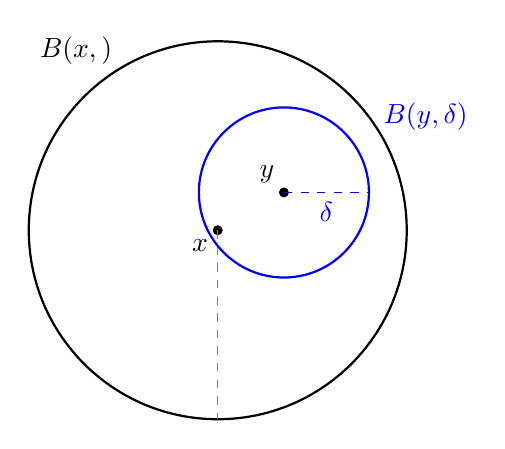
\begin{tikzpicture}[scale=1.2]
    % Big ball B(x, eps)
    \draw[thick] (0,0) circle (2);
    \fill (0,0) circle (1.5pt) node[below left] {$x$};
    \node at (-1.5, 1.9) {$B(x, \eps)$};
    % Draw radius
    \draw[dashed, gray] (0,0) -- (0,-2);
    \node[gray, right] at (0,-1) {$\eps$};

    % Point y inside
    \fill (0.7, 0.4) circle (1.5pt) node[above left] {$y$};

    % Small ball B(y, delta)
    \draw[thick, blue] (0.7, 0.4) circle (0.9);
    \node[blue] at (2.2, 1.2) {$B(y, \delta)$};

    % Draw delta radius
    \draw[dashed, blue] (0.7, 0.4) -- (1.6, 0.4);
    \node[blue, below] at (1.15, 0.4) {$\delta$};
\end{tikzpicture}
\end{center}
\end{notebox}

\begin{theorem}
A set $U$ is open in the metric topology on $X$ induced by $d$ if and only if for all $y \in U$, there exists $\delta > 0$ such that $B_d(y, \delta) \subseteq U$.
\end{theorem}

\begin{proof}
$(\Rightarrow)$ This follows directly from the definition of the topology generated by a basis.

$(\Leftarrow)$ For each $y \in U$, choose $\delta_y > 0$ such that $B_d(y, \delta_y) \subseteq U$. Then
\[
    U = \bigcup_{y \in U} B_d(y, \delta_y).
\]
Each $B_d(y, \delta_y)$ is open (it is a basis element), and an arbitrary union of open sets is open by the second topology axiom. Thus $U$ is open.
\end{proof}

\subsection{Closed Sets}

\begin{summarybox}
\textbf{Section Overview:} We define closed sets as complements of open sets and establish their dual properties (arbitrary intersections, finite unions). We then introduce closures, limit points, and isolated points, proving that $\overline{E} = E \cup E'$. Examples include the Cantor set and sets with isolated points. We also define boundedness (a metric-dependent property), convexity, and convergence of sequences in topological spaces.
\end{summarybox}

\begin{definition}
A set $C \subseteq X$ is \defn{closed} if its complement $X \setminus C$ is open.
\end{definition}

Properties of closed sets (dual to the open set axioms):
\begin{enumerate}
    \item $\emptyset$ and $X$ are closed.
    \item Arbitrary intersections of closed sets are closed.
    \item Finite unions of closed sets are closed.
\end{enumerate}

\begin{definition}
The \defn{closure} of a set $E \subseteq X$ is
\[
    \overline{E} = \bigcap \{ C \subseteq X \mid C \text{ is closed and } E \subseteq C \}.
\]
\end{definition}

\begin{theorem}
$x \in \overline{E}$ if and only if for every open set $U$ containing $x$, $U \cap E \neq \emptyset$. (We say $U$ is a \defn{neighborhood} of $x$.)
\end{theorem}

\begin{proof}
We prove the contrapositive: $x \notin \overline{E}$ if and only if there exists an open set $U$ containing $x$ with $U \cap E = \emptyset$.

$(\Rightarrow)$ If $x \notin \overline{E}$, then there exists a closed set $C \supseteq E$ with $x \notin C$. Let $U = X \setminus C$. Then $U$ is open, $x \in U$, and $U \cap E \subseteq U \cap C = \emptyset$.

$(\Leftarrow)$ If there exists an open set $U$ with $x \in U$ and $U \cap E = \emptyset$, then $C = X \setminus U$ is closed, $E \subseteq C$, and $x \notin C$. Thus $x \notin \overline{E}$.
\end{proof}

\begin{notebox}
\textbf{Proof by contrapositive.} To prove $P \Rightarrow Q$, it is equivalent to prove $\neg Q \Rightarrow \neg P$. This is often easier when the negation is more concrete to work with. In the proof above, showing ``$x \notin \overline{E}$ implies there exists an open set missing $E$'' is more direct than working with the original statement, because $x \notin \overline{E}$ hands us a specific closed set to work with. As a rule of thumb: if the statement you want to prove starts with ``for all,'' its contrapositive starts with ``there exists'' --- and existential statements are often easier to prove since you only need to produce one witness.

\begin{center}
\begin{tabular}{cc|cc}
$P$ & $Q$ & $P \Rightarrow Q$ & $\neg Q \Rightarrow \neg P$ \\
\hline
T & T & T & T \\
T & F & F & F \\
F & T & T & T \\
F & F & T & T \\
\end{tabular}
\end{center}
The columns for $P \Rightarrow Q$ and $\neg Q \Rightarrow \neg P$ are identical --- the two statements are logically equivalent.
\end{notebox}

\begin{definition}
A point $x$ is a \defn{limit point} of $E$ if every neighborhood $U$ of $x$ contains some $y \neq x$ with $y \in U \cap E$.
\end{definition}

\begin{theorem}
$\overline{E} = E \cup E'$, where $E'$ denotes the set of all \defn{limit points} of $E$.
\end{theorem}

\begin{proof}
$(\supseteq)$ If $x \in E$, then for every open $U$ containing $x$, we have $x \in U \cap E \neq \emptyset$, so $x \in \overline{E}$. If $x \in E'$, then every neighborhood $U$ of $x$ contains some $y \neq x$ with $y \in E$, so $U \cap E \neq \emptyset$, and thus $x \in \overline{E}$.

$(\subseteq)$ Suppose $x \in \overline{E}$ and $x \notin E$. Then for every neighborhood $U$ of $x$, $U \cap E \neq \emptyset$. Since $x \notin E$, the point witnessing $U \cap E \neq \emptyset$ must be some $y \neq x$ with $y \in E$. Thus $x \in E'$.
\end{proof}

\begin{notebox}
\textbf{Keeping $E$, $\overline{E}$, and $E'$ straight.}
\begin{itemize}
    \item $E$ --- the original set.
    \item $E'$ --- the \emph{limit points} (or \emph{derived set}) of $E$: points $x$ such that every neighborhood of $x$ contains some \emph{other} point of $E$. Note $x$ need not belong to $E$ itself.
    \item $\overline{E} = E \cup E'$ --- the \emph{closure} of $E$: the smallest closed set containing $E$. It includes the points of $E$ together with any ``boundary'' points that $E$ accumulates toward.
\end{itemize}
For example, if $E = (0,1) \subset \R$, then $E' = [0,1]$ (every neighborhood of $0$ or $1$ hits $(0,1)$), and $\overline{E} = E \cup E' = [0,1]$.
\end{notebox}

\begin{example}
\textbf{The Cantor set.} Let $C$ be the Cantor set, constructed by repeatedly removing the open middle third of each interval. Despite the intervals shrinking at each stage, the endpoints of every removed interval remain in $C$ and are limit points of $C$.

\begin{center}
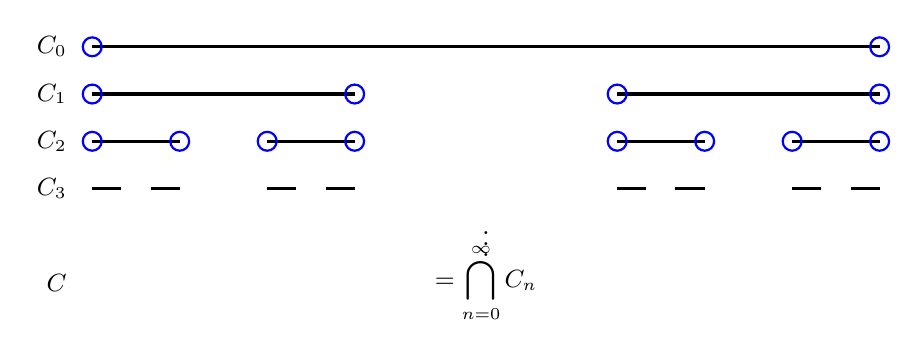
\begin{tikzpicture}[scale=10]
    % Stage 0: [0,1]
    \draw[very thick] (0,0) -- (1,0);
    \node[left] at (-0.02,0) {\small $C_0$};
    \draw[blue, thick] (0,0) circle (0.012);
    \draw[blue, thick] (1,0) circle (0.012);

    % Stage 1: [0,1/3] union [2/3,1]
    \draw[very thick] (0,-0.06) -- (0.3333,-0.06);
    \draw[very thick] (0.6667,-0.06) -- (1,-0.06);
    \node[left] at (-0.02,-0.06) {\small $C_1$};
    \draw[blue, thick] (0,-0.06) circle (0.012);
    \draw[blue, thick] (0.3333,-0.06) circle (0.012);
    \draw[blue, thick] (0.6667,-0.06) circle (0.012);
    \draw[blue, thick] (1,-0.06) circle (0.012);

    % Stage 2
    \draw[very thick] (0,-0.12) -- (0.1111,-0.12);
    \draw[very thick] (0.2222,-0.12) -- (0.3333,-0.12);
    \draw[very thick] (0.6667,-0.12) -- (0.7778,-0.12);
    \draw[very thick] (0.8889,-0.12) -- (1,-0.12);
    \node[left] at (-0.02,-0.12) {\small $C_2$};
    \draw[blue, thick] (0,-0.12) circle (0.012);
    \draw[blue, thick] (0.1111,-0.12) circle (0.012);
    \draw[blue, thick] (0.2222,-0.12) circle (0.012);
    \draw[blue, thick] (0.3333,-0.12) circle (0.012);
    \draw[blue, thick] (0.6667,-0.12) circle (0.012);
    \draw[blue, thick] (0.7778,-0.12) circle (0.012);
    \draw[blue, thick] (0.8889,-0.12) circle (0.012);
    \draw[blue, thick] (1,-0.12) circle (0.012);

    % Stage 3
    \draw[very thick] (0,-0.18) -- (0.0370,-0.18);
    \draw[very thick] (0.0741,-0.18) -- (0.1111,-0.18);
    \draw[very thick] (0.2222,-0.18) -- (0.2593,-0.18);
    \draw[very thick] (0.2963,-0.18) -- (0.3333,-0.18);
    \draw[very thick] (0.6667,-0.18) -- (0.7037,-0.18);
    \draw[very thick] (0.7407,-0.18) -- (0.7778,-0.18);
    \draw[very thick] (0.8889,-0.18) -- (0.9259,-0.18);
    \draw[very thick] (0.9630,-0.18) -- (1,-0.18);
    \node[left] at (-0.02,-0.18) {\small $C_3$};

    % Dots
    \node at (0.5,-0.24) {$\vdots$};
    \node[left] at (-0.02,-0.30) {\small $C$};
    \node at (0.5,-0.30) {\small $= \displaystyle\bigcap_{n=0}^{\infty} C_n$};
\end{tikzpicture}
\end{center}

The \textcolor{blue}{circled endpoints} at each stage are never removed --- they persist through every $C_n$ and thus belong to $C = \bigcap_{n=0}^{\infty} C_n$. Moreover, every neighborhood of such an endpoint contains points from the remaining intervals, making them limit points of $C$. In fact, $C$ is closed ($C = \overline{C}$) and every point of $C$ is a limit point: $C' = C$.
\end{example}

\begin{corollary}
$E$ is closed if and only if $E' \subseteq E$.
\end{corollary}

Points of $E \setminus E'$ are called \defn{isolated points}.

\begin{example}
Let $E = (0, \tfrac{1}{2}) \cup \{1\}$. The set of limit points is $E' = [0, \tfrac{1}{2}]$. Note that $1 \in E$ but $1 \notin E'$: for instance, the neighborhood $(\tfrac{3}{4}, \tfrac{5}{4})$ contains no point of $E$ other than $1$ itself. Thus $1$ is an isolated point of $E$.

Conversely, $0 \notin E$ and $\tfrac{1}{2} \notin E$, yet both are limit points: for any $\eps > 0$, the neighborhoods $(0 - \eps, 0 + \eps)$ and $(\tfrac{1}{2} - \eps, \tfrac{1}{2} + \eps)$ each contain points of $(0, \tfrac{1}{2}) \subseteq E$. The key takeaway: limit points can lie \emph{outside} the set, and points \emph{inside} the set need not be limit points.

\end{example}

\begin{example}
Consider the set $E = (0,1) \setminus \{\tfrac{1}{2}\}$: the open interval $(0,1)$ with a hole at $\tfrac{1}{2}$. Although $\tfrac{1}{2} \notin E$, it is a limit point of $E$: for any $\eps > 0$, the neighborhood $(\tfrac{1}{2} - \eps, \tfrac{1}{2} + \eps)$ contains points of $E$ other than $\tfrac{1}{2}$. Being in the set and being a limit point are independent properties.
\end{example}

\begin{definition}
A subset $E$ of a metric space $(X, d)$ is \defn{bounded} if there exist $x \in X$ and $M > 0$ such that $E \subseteq B(x, M)$, i.e., $d(x, y) < M$ for all $y \in E$.
\end{definition}

\begin{remark}
Boundedness is a metric-dependent property, not a topological one. The same set can be bounded under one metric and unbounded under another. For example, $\R$ with the usual metric $d(x,y) = |x - y|$ is unbounded. However, define the \emph{bounded metric} $\bar{d}(x,y) = \min(|x-y|, 1)$. This induces the same topology on $\R$ (the same sets are open), but now $\R$ is bounded: $\bar{d}(x,y) \leq 1$ for all $x, y$, so $\R \subseteq B(0, 2)$. Since two metrics can generate the same topology yet disagree on boundedness, boundedness is not a topological invariant --- it depends on the choice of metric.
\end{remark}

\begin{definition}
A set $E \subseteq \R$ is \defn{convex} if for all $x, y \in E$ and for all $\lambda \in (0,1)$,
\[
    \lambda x + (1 - \lambda) y \in E.
\]

\begin{center}
\begin{tikzpicture}[scale=1.5]
    % Line segment
    \draw[thick, blue] (0,0) -- (4,2);

    % Endpoints
    \fill (0,0) circle (1.5pt) node[below left] {$x$};
    \fill (4,2) circle (1.5pt) node[above right] {$y$};

    % Midpoint p = lambda x + (1-lambda) y
    \fill[red] (2,1) circle (1.5pt);
    \node[above left, red] at (2,1) {$p = \lambda x + (1-\lambda)y$};
\end{tikzpicture}
\end{center}
\end{definition}

\begin{definition}
A sequence $(x_n)$ in a topological space $X$ \defn{converges} to $y \in X$ if for every neighborhood $U$ of $y$, there exists $N \in \N$ such that for all $n \geq N$, $x_n \in U$.
\end{definition}

\begin{theorem}
The product topology on $\R^n = \R \times \cdots \times \R$ equals the metric topology induced by the Euclidean metric.
\end{theorem}

\begin{proof}
We show both topologies have the same open sets by showing each basis element of one is open in the other.

\textbf{Product basis elements are open in the metric topology.} A basic open set in the product topology is $(a_1, b_1) \times \cdots \times (a_n, b_n)$. Let $x = (x_1, \dots, x_n)$ be a point in this set. For each $i$, choose $\eps_i = \min(x_i - a_i, \, b_i - x_i) > 0$. Set $\eps = \min(\eps_1, \dots, \eps_n) > 0$. Then $B(x, \eps) \subseteq (a_1, b_1) \times \cdots \times (a_n, b_n)$, since if $d(x, y) < \eps$ then $|x_i - y_i| \leq d(x, y) < \eps \leq \eps_i$ for each $i$, so $y_i \in (a_i, b_i)$.

\textbf{Open balls are open in the product topology.} Let $x \in B(y, \eps)$ and set $\delta = \eps - d(x, y) > 0$. Consider the product of intervals
\[
    U = \left(x_1 - \tfrac{\delta}{\sqrt{n}}, \, x_1 + \tfrac{\delta}{\sqrt{n}}\right) \times \cdots \times \left(x_n - \tfrac{\delta}{\sqrt{n}}, \, x_n + \tfrac{\delta}{\sqrt{n}}\right).
\]
This is open in the product topology, $x \in U$, and for any $z \in U$ we have
\[
    d(x, z) = \sqrt{\sum_{i=1}^n (x_i - z_i)^2} < \sqrt{n \cdot \tfrac{\delta^2}{n}} = \delta,
\]
so $z \in B(x, \delta) \subseteq B(y, \eps)$. Thus $U \subseteq B(y, \eps)$, and $B(y, \eps)$ is open in the product topology.
\end{proof}

\begin{theorem}
If $p \in E'$, then every neighborhood $U$ of $p$ contains infinitely many points of $E$.
\end{theorem}

\begin{proof}
By contradiction. Suppose $U$ is a neighborhood of $p$ containing only finitely many points $q_1, \dots, q_n \in U \cap E$ with $q_i \neq p$. Let $r = \min_{1 \leq i \leq n} d(p, q_i) > 0$. Then $B(p, r)$ contains no point of $E$ other than $p$ itself. But $p \in E'$, so every neighborhood of $p$ must contain some $y \neq p$ with $y \in E$ --- a contradiction.
\end{proof}

\end{document}
